\chapter{ALL ABOUT STEINER TREE} \label{ch_prelim}
% %Chapter 2
% %%%%%%%%%%%%%%%%%%%%%%%%%%%%%%%%%%%%%%%%%%%%%%%%%%%%%%%%%%%%%%%%%%%%%%
In this chapter, we are presenting all about the Steiner tree problems. In this we will present, what are the properties of the Steiner tree and types of the Steiner tree, which are the algorithms for the different type of Steiner tree and their approximation algorithms.
\section{Steiner Tree}
 The Steiner Tree in a given graph $G = (V,E)$ is a tree that cover all the terminal vertices of the graph with minimum cost, terminals are the subset of the vertices which are required in the connection, i.e., have to be cover in the minimum spanning tree.
 In this section we define and give different type of Steiner tree problems.
\section{Types of Steiner Trees problems}
 Based on the applications and uses the Steiner tree are of the different types. For example, if a Steiner tree is applied in the VLSI network, then this type of Steiner tree so called as the terminal Steiner tree. In this section, we will discuss a few types of Steiner tree Problems.

\subsection{Euclidean Steiner Tree}
 The Euclidean Steiner Problem(ESP) was well researched by Zacharis, the origin of ESP is often traced back to Fermat(1601-1665) 
 who proposed the following problem: We are given some terminal points in the 2-dimensional space and some optional points. Here we considering the cost of connecting the points is same as the distance between the points. Find a point in the plane that sum the connection of minimum distance, and point is in such a way that the sum of whose distances from three given points should be minimal.
  This problem will be referred to as the Fermat problem. In figure 2.1 three points are shown in the Euclidean plane, if we connect these point with help of a Steiner point(shown as hollow in figure) then we will get a tree that covers all these points with minimum distance $\sqrt{3}$. 

  A solution for this problem is given by torricelli in 1640, he gave solution by using some geometric triangle for this problem. He propose that, if we draw three circles using circumscribing of equilateral triangles sides for construction of the circle, these circle meat at point that point called as called the Torricelli point. In figure 2.2, in triangle, a Torricelli point is formed after the intersection of three circles. The circle are drowned at the edges of the equilateral triangle every circle pass through the two points of side of the triangle and the intersection point of these three circles is so called Torricelli point. The distance from the Torricelli point and the give point is called Euclidean distance and the sum of all the distance is minimum.

   Here in this figure 2.1, shown that the solution of the 3 points problem with the Torricelli method, if we found a Torricelli point, we can draw edges having an equal distance from this point to the other point. In this figure 2.1, point form a triangle, if we form a minimum weight tree from this triangle the total cost of that minimum spanning tree will be 2 which is not the minimum cost of covering all points in the plane, and if we form a Steiner minimum tree by taking the Steiner point as the center of these point, then we are getting a tree that covers all points with minimum distance this is so called Steiner tree.

    
\begin{figure}
\centering
\begin{subfigure}{.5\textwidth}
  \centering
  \begin{tikzpicture}[shorten >=1pt, auto, node distance=2cm, ultra thick,
            node_style/.style={circle,draw=black,minimum size = 10pt,font=\sffamily\Large\bfseries},
            edge_style/.style={draw=black, ultra thick}]
    % \node[node_style] (v1) at (0,0)  {a};
    \node[node_style,fill=black!500] (v2) at (-2,-1) {};
    \node[node_style,fill=black!500] (v3) at (2,-1)  {};
    \node[node_style,fill=black!500] (v4) at (0,2) {};
    \end{tikzpicture}
  
  % \includegraphics[width=.4\linewidth]{image1}
  \caption{}
  \label{fig:sub1}
\end{subfigure}%
\begin{subfigure}{.5\textwidth}
  \centering
  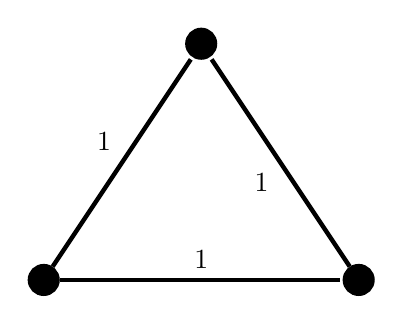
\begin{tikzpicture}[shorten >=1pt, auto, node distance=2cm, ultra thick,
            node_style/.style={circle,draw=black,minimum size = 10pt,font=\sffamily\Large\bfseries},
            edge_style/.style={draw=black, ultra thick}]
    % \node[node_style] (v1) at (0,0)  {a};
    \node[node_style,fill=black!500] (v2) at (-2,-1) {};
    \node[node_style,fill=black!500] (v3) at (2,-1)  {};
    \node[node_style,fill=black!500] (v4) at (0,2) {};

    \draw[edge_style]  (v2) edge node{1} (v3);
    \draw[edge_style]  (v2) edge node{1} (v4);
    \draw[edge_style]  (v3) edge node{1} (v4);
    \end{tikzpicture}
  
  % \includegraphics[width=.4\linewidth]{image1}
  \caption{}
  \label{fig:sub2}
\end{subfigure}
% \caption{A figure with two subfigures}
% \label{fig:test}
% \end{figure}
\\

% \begin{figure}
\centering
\begin{subfigure}{.5\textwidth}
  \centering
  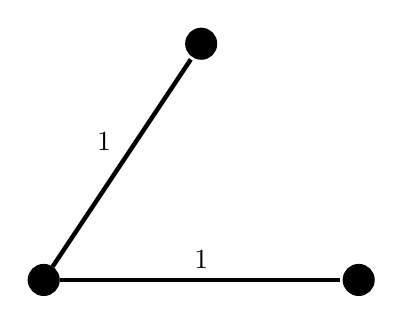
\begin{tikzpicture}[shorten >=1pt, auto, node distance=2cm, ultra thick,
            node_style/.style={circle,draw=black,minimum size = 10pt,font=\sffamily\Large\bfseries},
            edge_style/.style={draw=black, ultra thick}]
    % \node[node_style] (v1) at (0,0)  {a};
    \node[node_style,fill=black!500] (v2) at (-2,-1) {};
    \node[node_style,fill=black!500] (v3) at (2,-1)  {};
    \node[node_style,fill=black!500] (v4) at (0,2) {};
    \draw[edge_style]  (v2) edge node{1} (v4);
    \draw[edge_style]  (v2) edge node{1} (v3);
    % \draw[edge_style]  (v5) edge node{10} (v4);
    \end{tikzpicture}
  
  % \includegraphics[width=.4\linewidth]{image1}
  \caption{}
  \label{fig:sub1}
\end{subfigure}%
\begin{subfigure}{.5\textwidth}
  \centering
  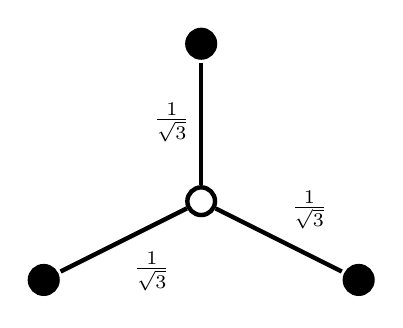
\begin{tikzpicture}[shorten >=1pt, auto, node distance=2cm, ultra thick,
            node_style/.style={circle,draw=black,minimum size = 10pt,font=\sffamily\Large\bfseries},
            edge_style/.style={draw=black, ultra thick}]
    \node[node_style] (v1) at (0,0)  {};
    \node[node_style,fill=black!100] (v2) at (-2,-1) {};
    \node[node_style,fill=black!500] (v3) at (2,-1)  {};
    \node[node_style,fill=black!500] (v4) at (0,2) {};
    \draw[edge_style]  (v1) edge node{$\frac{1}{\sqrt{3}}$} (v2);
    \draw[edge_style]  (v1) edge node{$\frac{1}{\sqrt{3}}$} (v3);
    \draw[edge_style]  (v1) edge node{$\frac{1}{\sqrt{3}}$} (v4);
    \end{tikzpicture}
  
  % \includegraphics[width=.4\linewidth]{image1}
  \caption{}
  \label{fig:sub2}
\end{subfigure}
\caption{(a) three points are given in the euclidean plane. (b) these point form triangle suppose edges length is 1 for each. (c) minimum spanning tree of cost 2. (d) Steiner tree form using one Steiner point}
\label{fig:test}
\end{figure}

 \begin{figure}
      \centering
    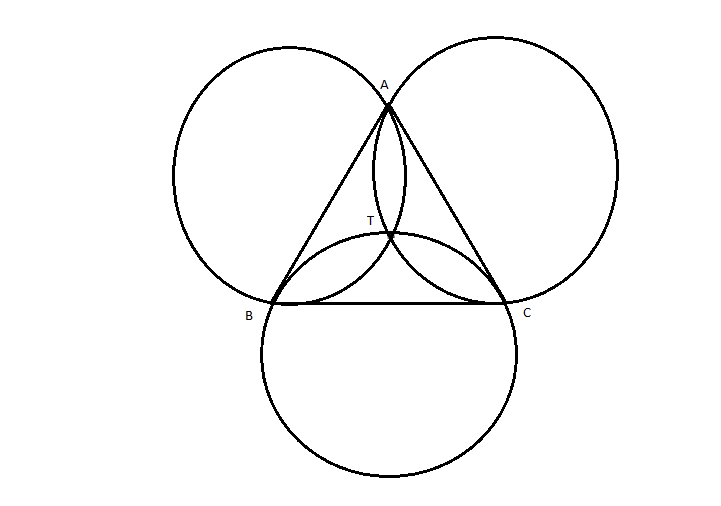
\includegraphics[scale = 0.8]{torr.png}
  \caption{A triangle ABC, and Torricelli Point T (Black dot at the center of the triangle ABC)} intersection of all the circle.
\end{figure}

 Characteristics of this Torricelli point that it always lies inside the triangle and the distance sum from all other point triangle corner to the torricelli point is minimum. If triangle is equilateral triangle than $\angle$ ATC = $\angle$ BTC = $\angle$ CTA = $120$. As Shown in figure 2.2, Circle are draw by taking center as the outside intersection point of arch drown by taking the corner of the triangle edge as a center, by taking that intersection point as center and  draw a circle which passes through the end points of edges, this process is done for all the three circle, the intersection point of these three circle is so called Steiner point or torricelli point.   

 
\subsection{Rectilinear Steiner Problem}
A Steiner tree, whose spanning tree overs a set of points in the collection by using vertical and horizontal lines which covers the points in the given space is called rectilinear tree. These sets of lines are called Steiner trees. The Length of a tree is the weight sum of its lines, and a rectilinear Steiner minimal tree(RSMT) is a tree of minimum length. According the statement by Hanan's we can find the number of Steiner tree exist in a grid, that having the points. This can be drown by horizontal and vertical line than can be form by connecting the set of points that are presents in the plane ~\cite{shen}.

Rectilinear minimum Steiner tree problem is a one of the problem in the geometric plane for the Steiner tree problem, for that we have to replaced euclidean distance by rectilinear distance that form a grid like structure. Given the points there is a interconnections between the points in fashion of horizontal and vertical lines. This arises the application of Steiner tree VLSI design, because in VLSI design there is a linear relationship between the wire-length and wiring area.

In figure 2.3(a), grid structure is given to the four points lies in the rectilinear plane, suppose that the distance from one grid to another grid is 1, from both way horizontal or vertical. In figure 2.3(b), a minimum spanning tree is formed by using these points, the cost of forming minimum spanning tree will be 6, this cost is not minimal cost of covering all the points in rectilinear plane. In figure 2.3(c), we are using one Steiner point(show as hollow) to connect all the required vertices, than the cost of covering all the points will be 4 which is minimum cost of covering all the points. 
 \begin{figure}
      \centering
    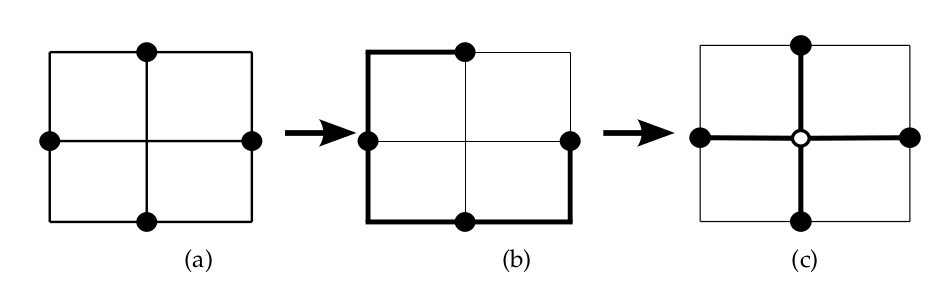
\includegraphics[scale = 0.4]{rec.png}
  \caption{(a) Grid having four terminal point int rectilinear plane (b) minimum spanning tree of cost 6 using all four points (c) minimum Steiner tree of cost 4}
\end{figure}

\subsection{Steiner Tree Problems in Network}
This problem is the combinatorial version of the Euclidean problem for Steiner tree. If $G$ is not connected and terminals appear in 
at least two components, then there is no solution for the Steiner problem. If G is not connected but all terminals appears in one component, then the remaining components can be disregarded and we can get the solution for the by using only the terminals that are present in the component. For this problem in the network by using Steiner tree, it is assumed that the $G$ is connected graph. The Problem of Steiner tree in networks was originally formulated by Hakimiand independently by levinin 1971. After that this problem received considerable attention for the research in the network.\\

 \begin{tabular}{|ll|} 
 \hline
 \multicolumn{ 2}{|l|}{\problemfontbold{Steiner Tree Problem in Network}} \\
 \emph{INPUT} & \begin{minipage}[t]{0.8\columnwidth}
 A undirected graph G = $(V,E)$, edge costs c:E$\rightarrow$ $\mathbb{R}_{\geq 0}$, and a nodes $S \subseteq V$,  $S$ is the subset if vertices, called required nodes.
 \end{minipage} \\
 \emph{OUTPUT} & \begin{minipage}[t]{0.8\columnwidth}
 A Steiner Tree $T_s$, Such that there is a path between every pair of terminals.\\
 \end{minipage}
 \\
 \hline
 \end{tabular}
 \\

\subsection{Prize-Collecting Steiner Tree(PCST)}
The Prize collecting Steiner tree(PCST) in a given undirected graph G, with edges cost and vertex profits. In PCST we form a Steiner tree by using terminal vertices such that it minimizing total sum of the edge's weight in the Steiner tree plus the profit of all the vertices which are not in the Steiner tree.

\begin{tabular}{|ll|} 
 \hline
 \multicolumn{ 2}{|l|}{\problemfontbold{Prize-Collecting Steiner Tree(PCST)}} \\
 \emph{INPUT} & \begin{minipage}[t]{0.8\columnwidth}
 A undirected connected graph $G$ = $(V,E)$ with edge costs $c:E\rightarrow \mathbb{R}_{\geq 0}$, and a $|S|$ nodes $S \subseteq V$,  $|S|$ is so called terminal nodes and $p$ is vertex profit.
 \end{minipage} \\
 \emph{OUTPUT} & \begin{minipage}[t]{0.8\columnwidth}
 A Steiner Tree $T_s$ = $(V_s,E_s)$ of G, $E_s$ $\subseteq$E, that minimize the objective function c(s) =$\sum_{v_{\notin V_s}}p(V)$ + $\sum_{E_{\in E_s}}c(E)$  .\\
 \end{minipage}
 \\
 \hline
 \end{tabular}
 \\


\section{Approximation Algorithm for Steiner Tree}

Here we are presenting the approximation algorithm from a graph $G$ for finding the Steiner tree. A graph $G$ is given with edges weight and a vertex set $|S|$ which, we called as the terminal nodes. Sequence of vertices $(v_1,v_2,v_3 \dots v_k)$ is known as the path in the graph. The Weighted sum of all the edges which are present in the path is known as the weight of the path. A spanning tree is the tree that cover all the vertices of the graph, if the weight of a path is minimum than this tree is so called as the minimum spanning tree. If we applied some conditions on this like, we have to cover some particular nodes, and have to find the minimum distance between these nodes, then these type of cases comes under the category of the Steiner tree problems, in that we have to cover all the terminals, if all the terminals cover by a tree with minimum weight, i.e., there is no other optimal weighted tree which have less weight than of that, this type of tree so called as the minimum Steiner tree.

 Finding a minimum Steiner tree in a graph $G$ and $S$ is the NP-complete problem. So have to think about some approximation solution for these problems. An approximation algorithm best known for Steiner tree problems. We start with a heuristic algorithm that can be use for finding the Steiner tree from a given graph ~\cite{markowsky}. We will show the Steiner tree algorithm and their explanation by taking some graph as an example.

\subsection{Heuristic Algorithm :-}
Heuristic Algorithm for construct a Steiner tree from a graph ~\cite{markowsky}.\\
Given a connected undirected graph $G$, and edges weight or cost is the minimum distance $d$ between two vertices $v_i$ and $v_j$ if there is a edge. We are given some require vertices $S$, $S$ is the subset of vertices $S \subseteq V$. Heuristic algorithm for the Steiner tree following. A path is a sequence of vertices, $(v_1,v_2,v_3 \dots, v_n)$, a path from a vertex $v_1$ to $v_n$ going through the vertices $(v_2,v_3 \dots, v_{n-1})$~\cite{karger}. A symbol ($u$ $\leadsto$ $v$) is used for path representation from $u$ to $v$ (if there exits a edge between ($u$,$v$)). A simple path is a path in which all the vertices are distinct. Sum of the path is the sum of weights of all the edges which are used in the path. A Shortest path is the path between the vertices $v_1$ to $v_n$ whose path sum is minimum among all the possible paths from $v_1$ to $v_n$. A loop is a path, $(v_1,v_2,v_3 \dots, v_n)$, such that $v_1$ = $v_n$. Here we are presenting algorithm $algo2$ for finding the Steiner tree in given graph $G$ as a input.\\ A Steiner tree is a tree that cover all the required vertices with the minimum distance. This algorithm $algo2$ is the 3 steps algorithm for finding the Steiner tree. The Steiner tree produced by algorithm suggested heuristic algorithm is not necessarily minimal. However, it will be shown that the total distance $D_H$ will not be very far from the $D_{MIN}$, $D_{MIN}$ is the total distance of the minimum Steiner tree. We have shown approximation ratio 2$\Big(1-\frac{1}{|S|}\Big)$ in $Algo1$, where $|S|$ is the number of terminals in the graph. In fact, we have also shown one more approximation ratio $D_H$/$D_{MIN}$ $\leq$ 2$\Big(1 - \frac{1}{l} \Big)$, where l is the  number of leaves in the minimal Steiner tree~\cite{markowsky}.



\begin{tabular}{|ll|} 
 \hline
 \multicolumn{ 2}{|l|}{\problemfontbold{Algorithm 1:- }} \\
 \emph{INPUT} & \begin{minipage}[t]{0.9\columnwidth}
 A undirected graph $G = (V,E)$, distance $d$ between the vertices $v_i$ and $v_j$, i.e., edge weight $d$ and a subset of nodes $S\subseteq V$,  $S$ is called as required vertex.
 \end{minipage} \\
 \emph{OUTPUT} & \begin{minipage}[t]{0.8\columnwidth}
 A Steiner Tree $T_s$ = $(V_s,E_s)$ of $G$ and $S$.\\
 \end{minipage}\\
 \emph{Step 1.} & \begin{minipage}[t]{0.9\columnwidth}
 First take the given graph $G$ and the required vertices($S$), and construct a complete distance graph $G_1$=$(V_1,E_1)$.\\
 \end{minipage}
 \\
 \emph{Step 2.} & \begin{minipage}[t]{0.9\columnwidth}
 From that graph $G_1$ find a minimum spanning tree, $T_1$. there may be chance that more than one minimum spanning tree are possible, than choose arbitrary one of the minimum spanning tree.\\
 \end{minipage}
 \\
 \emph{Step 3.} & \begin{minipage}[t]{0.9\columnwidth}
 Construct the sub-graph $G_s$, by using the graph $G$ by replacing each edges by it's shortest path in $G$, according to the edges present in the minimum spanning tree from step 2.(If more than one shortest paths are their choose all shortest path).\\
 \end{minipage}
 \\
  \emph{Step 4.} & \begin{minipage}[t]{0.9\columnwidth}
 Find minimum spanning tree from that sub-graph $G_s$.(If more that one minimum spanning tree are presents, then any one minimum spanning tree from that).\\
 \end{minipage}
 \\
 \emph{Step 5.} & \begin{minipage}[t]{0.9\columnwidth}
 Now delete all the unnecessary edges which are not connecting the required vertices (S), final tree is so called as the Steiner tree.\\
 \end{minipage}
 \\
 \hline
 \end{tabular}
 \\

In this algorithm run time taken by each Step is as, Step 1 run time $O(|S||V|^2)$, Step 2 can be done in $O(|S|^2)$ time, Step 3 can be done in the order of $O(|V|)$ time, step 4 could be done in $O(|V|^2)$ time and time taken by the Step 5 will of order $O(|V|)$ time. Here in these steps only first step is taking more running time then the other steps. So can say the overall running time complexity for this algorithm will be $O(|S||V|^2)$ ~\cite{markowsky}.  \\
With the help of an example, we are explaining each and every steps of this heuristic algorithm.\\
Example:


\begin{figure}
\begin{center}
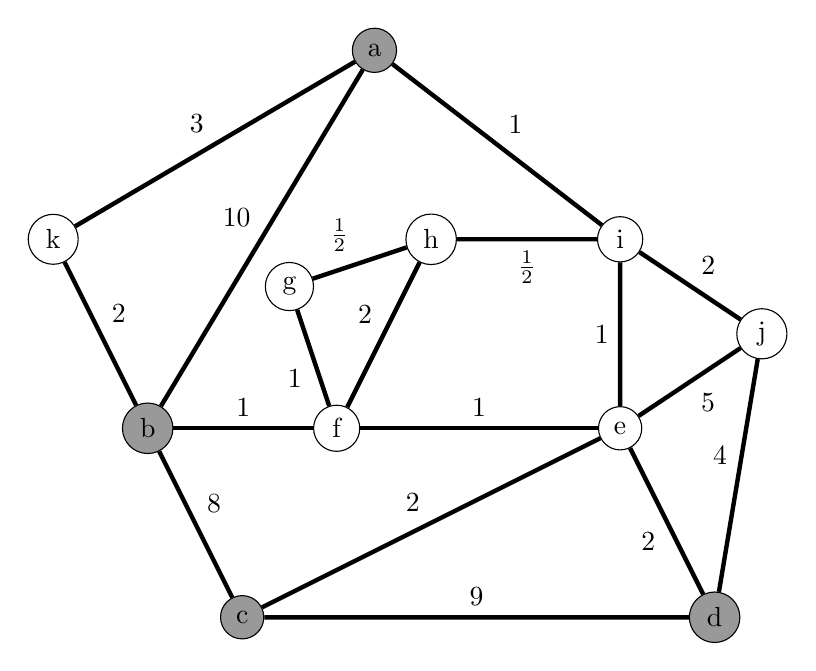
\begin{tikzpicture}[scale=1.2, auto, node distance=2cm,
   node_style/.style={circle,draw=black},
   edge_style/.style={draw=black, ultra thick}]

    \node[node_style, fill=black!40] (v1) at (0.4,4) {a};
    \node[node_style, fill=black!40] (v2) at (-2, 0) {b};
    \node[node_style] (v11) at (-3, 2) {k};
    \node[node_style, fill=black!40] (v3) at (-1,-2)  {c};
    \node[node_style, fill=black!40] (v4) at (4,-2)  {d};

    \node[node_style] (v5) at (3,0) {e};
    \node[node_style] (v6) at (0,0)  {f};
    \node[node_style] (v7) at (-0.5,1.5) {g};
    \node[node_style] (v8) at (1,2) {h};
    \node[node_style] (v9) at (3,2)  {i};
    \node[node_style] (v10) at (4.5,1) {j};
    % \node[node_style] (v10) at (2,-2) {l};
    % \node[node_style,fill=black!40] (v11) at (4,-3) {c};
    % \node[node_style,fill=black!40] (v12) at (3,2)  {e};
    \draw[edge_style]  (v2) edge node{1} (v6);
    \draw[edge_style]  (v2) edge node{10} (v1);
    \draw[edge_style]  (v2) edge node{8} (v3);
    \draw[edge_style]  (v1) edge node{1} (v9);
    \draw[edge_style]  (v9) edge node{$\frac{1}{2}$} (v8);
    \draw[edge_style]  (v7) edge node{$\frac{1}{2}$} (v8);
    \draw[edge_style]  (v6) edge node{1} (v7);
    \draw[edge_style]  (v6) edge node{1} (v5);
    \draw[edge_style]  (v4) edge node{2} (v5);
    \draw[edge_style]  (v3) edge node{9} (v4);
    % \draw[edge_style]  (v3) edge node{8} (v2);
    \draw[edge_style]  (v3) edge node{2} (v5);
    \draw[edge_style]  (v5) edge node{1} (v9);
    \draw[edge_style]  (v9) edge node{2} (v10);
    \draw[edge_style]  (v10) edge node{5} (v5);
    \draw[edge_style]  (v4) edge node{4} (v10);
    \draw[edge_style]  (v6) edge node{2} (v8);
    \draw[edge_style]  (v11) edge node{3} (v1);
    \draw[edge_style]  (v11) edge node{2} (v2);
    
    
    
    \end{tikzpicture}
    % \caption{\small \sl Torricelli point X \label{fig:sccEx} }
    \caption{Connected weighted Graph $G$, with Steiner vertices(hollow), and 4 terminal vertices(dark)}
    \end{center}
    
    % \caption{\small \sl  }
    \end{figure}

 \begin{figure}
\centering
\begin{subfigure}{.5\textwidth}
  \centering
      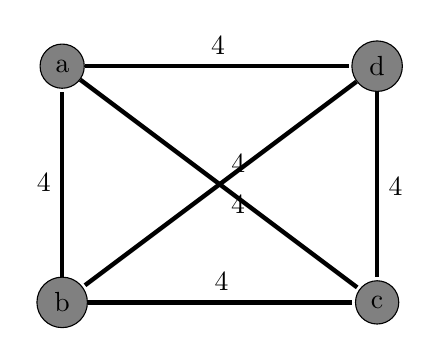
\begin{tikzpicture}[shorten >=1pt, auto, node distance=20cm,
            node_style/.style={circle,draw=black,minimum size = 10pt},
            edge_style/.style={draw=black, ultra thick}]
    % \node[node_style,fill=black!50] (v1) at (0,4)  {a};
    \node[node_style,fill=black!50] (v2) at (-2,-1) {b};
    \node[node_style,fill=black!50] (v3) at (2,-1)  {c};
    \node[node_style,fill=black!50] (v4) at (2,2) {d};
    \node[node_style,fill=black!50] (v5) at (-2,2) {a};
    
    \draw[edge_style]  (v2) edge node{4} (v5);
    \draw[edge_style]  (v2) edge node{4} (v3);
    \draw[edge_style]  (v5) edge node{4} (v4);
    \draw[edge_style]  (v4) edge node{4} (v3);
    \draw[edge_style]  (v5) edge node{4} (v3);
    \draw[edge_style]  (v4) edge node{4} (v2);
    \end{tikzpicture}

  
  % \includegraphics[width=.4\linewidth]{image1}
  \caption{A complete graph of $G$ using terminals nodes, with minimum edges weight between terminals}
  % \label{fig:sub1}
\end{subfigure}%
\begin{subfigure}{.5\textwidth}
  \centering
  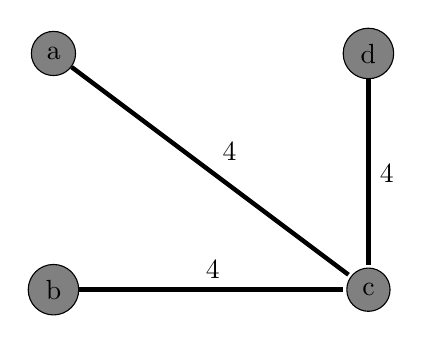
\begin{tikzpicture}[shorten >=1pt, auto, node distance=20cm,
            node_style/.style={circle,draw=black,minimum size = 10pt},
            edge_style/.style={draw=black, ultra thick}]
    % \node[node_style,fill=black!50] (v1) at (0,4)  {a};
    \node[node_style,fill=black!50] (v2) at (-2,-1) {b};
    \node[node_style,fill=black!50] (v3) at (2,-1)  {c};
    \node[node_style,fill=black!50] (v4) at (2,2) {d};
    \node[node_style,fill=black!50] (v5) at (-2,2) {a};
     \draw[edge_style]  (v2) edge node{4} (v3);
  
     \draw[edge_style]  (v4) edge node{4} (v3);
     \draw[edge_style]  (v5) edge node{4} (v3);
    % \draw[edge_style]  (v4) edge node{4} (v2);
    \end{tikzpicture}
  
  % \includegraphics[width=.4\linewidth]{image1}
  \caption{Minimum spanning tree from complete graph}
  % \label{fig:sub2}
\end{subfigure}


%%%%%%%%%%%%%%%%%%%%%%%%%%%%%%%%%%%%%%%%%%%%%%%%%%%%%%%%%%%%%%%%%%%%%%%%%%%%%%%%%

% \begin{figure}
\begin{center}
    % \caption{\small \sl Torricelli point X \label{fig:sccEx} }
    \end{center}
    

 % \begin{figure}
\centering
\begin{subfigure}{.5\textwidth}
  \centering
      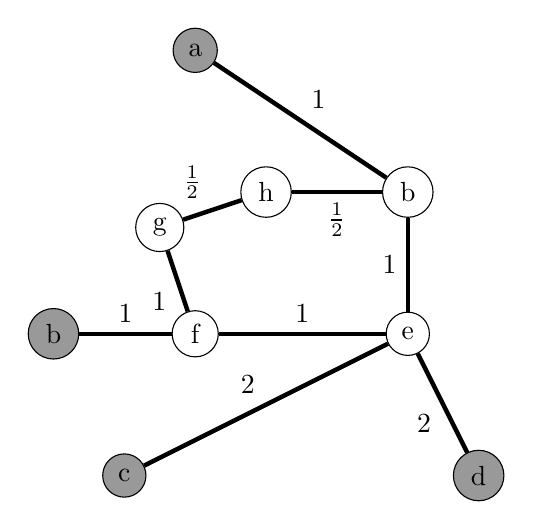
\begin{tikzpicture}[scale=0.9, auto, node distance=2cm,
   node_style/.style={circle,draw=black},
   edge_style/.style={draw=black, ultra thick}]

    \node[node_style, fill=black!40] (v1) at (0,4) {a};
    \node[node_style, fill=black!40] (v2) at (-2, 0) {b};
    \node[node_style, fill=black!40] (v3) at (-1,-2)  {c};
    \node[node_style, fill=black!40] (v4) at (4,-2)  {d};

    \node[node_style] (v5) at (3,0) {e};
    \node[node_style] (v6) at (0,0)  {f};
    \node[node_style] (v7) at (-0.5,1.5) {g};
    \node[node_style] (v8) at (1,2) {h};
    \node[node_style] (v9) at (3,2)  {b};
    % \node[node_style] (v10) at (2,-2) {l};
    % \node[node_style,fill=black!40] (v11) at (4,-3) {c};
    % \node[node_style,fill=black!40] (v12) at (3,2)  {e};
    \draw[edge_style]  (v2) edge node{1} (v6);
    % \draw[edge_style]  (v2) edge node{10} (v1);
    % \draw[edge_style]  (v2) edge node{8} (v3);
    \draw[edge_style]  (v1) edge node{1} (v9);
    \draw[edge_style]  (v9) edge node{$\frac{1}{2}$} (v8);
    \draw[edge_style]  (v7) edge node{$\frac{1}{2}$} (v8);
    \draw[edge_style]  (v6) edge node{1} (v7);
    \draw[edge_style]  (v6) edge node{1} (v5);
    \draw[edge_style]  (v4) edge node{2} (v5);
    % \draw[edge_style]  (v3) edge node{9} (v4);
    % \draw[edge_style]  (v3) edge node{8} (v2);
    \draw[edge_style]  (v3) edge node{2} (v5);
    \draw[edge_style]  (v5) edge node{1} (v9);
    \end{tikzpicture}


  
  % \includegraphics[width=.4\linewidth]{image1}
  \caption{A subgraph of graph $G$}
  % \label{fig:sub1}
\end{subfigure}%
\begin{subfigure}{.5\textwidth}
  \centering
  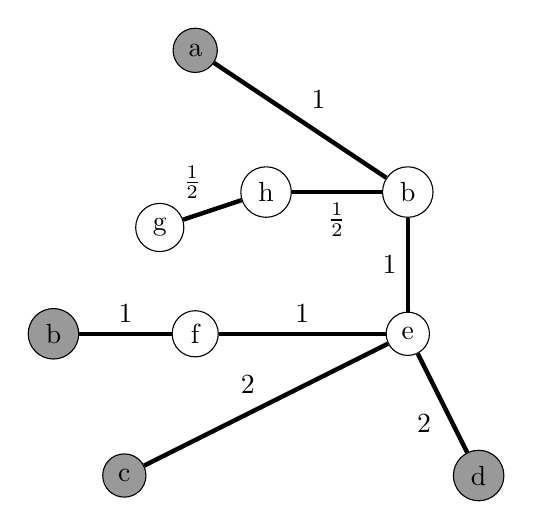
\begin{tikzpicture}[scale=0.9, auto, node distance=2cm,
   node_style/.style={circle,draw=black},
   edge_style/.style={draw=black, ultra thick}]

    \node[node_style, fill=black!40] (v1) at (0,4) {a};
    \node[node_style, fill=black!40] (v2) at (-2, 0) {b};
    \node[node_style, fill=black!40] (v3) at (-1,-2)  {c};
    \node[node_style, fill=black!40] (v4) at (4,-2)  {d};

    \node[node_style] (v5) at (3,0) {e};
    \node[node_style] (v6) at (0,0)  {f};
    \node[node_style] (v7) at (-0.5,1.5) {g};
    \node[node_style] (v8) at (1,2) {h};
    \node[node_style] (v9) at (3,2)  {b};
    % \node[node_style] (v10) at (2,-2) {l};
    % \node[node_style,fill=black!40] (v11) at (4,-3) {c};
    % \node[node_style,fill=black!40] (v12) at (3,2)  {e};
    \draw[edge_style]  (v2) edge node{1} (v6);
    % \draw[edge_style]  (v2) edge node{10} (v1);
    % \draw[edge_style]  (v2) edge node{8} (v3);
    \draw[edge_style]  (v1) edge node{1} (v9);
    \draw[edge_style]  (v9) edge node{$\frac{1}{2}$} (v8);
    \draw[edge_style]  (v7) edge node{$\frac{1}{2}$} (v8);
    % \draw[edge_style]  (v6) edge node{1} (v7);
    \draw[edge_style]  (v6) edge node{1} (v5);
    \draw[edge_style]  (v4) edge node{2} (v5);
    % \draw[edge_style]  (v3) edge node{9} (v4);
    % \draw[edge_style]  (v3) edge node{8} (v2);
    \draw[edge_style]  (v3) edge node{2} (v5);
    \draw[edge_style]  (v5) edge node{1} (v9);
    
    \end{tikzpicture}

  
  % \includegraphics[width=.4\linewidth]{image1}
  \caption{Minimum spanning tree from subgraph}
  % \label{fig:sub2}

\end{subfigure}
\end{figure}
% \label{fig:sccEx}



\begin{figure}
\begin{center}
\begin{subfigure}{.5\textwidth}

  \centering
  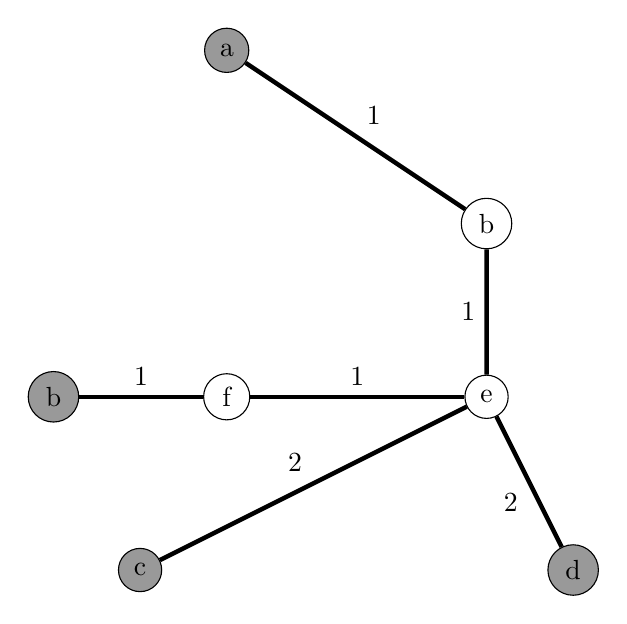
\begin{tikzpicture}[scale=1.1, auto, node distance=2cm,
   node_style/.style={circle,draw=black},
   edge_style/.style={draw=black, ultra thick}]

    \node[node_style, fill=black!40] (v1) at (0,4) {a};
    \node[node_style, fill=black!40] (v2) at (-2, 0) {b};
    \node[node_style, fill=black!40] (v3) at (-1,-2)  {c};
    \node[node_style, fill=black!40] (v4) at (4,-2)  {d};

    \node[node_style] (v5) at (3,0) {e};
    \node[node_style] (v6) at (0,0)  {f};
    \node[node_style] (v9) at (3,2)  {b};
    \draw[edge_style]  (v2) edge node{1} (v6);
    \draw[edge_style]  (v1) edge node{1} (v9);
    \draw[edge_style]  (v6) edge node{1} (v5);
    \draw[edge_style]  (v4) edge node{2} (v5);
    \draw[edge_style]  (v3) edge node{2} (v5);
    \draw[edge_style]  (v5) edge node{1} (v9);
    \end{tikzpicture}

  
  % \includegraphics[width=.4\linewidth]{image1}
  \caption{Terminal Steiner tree of a Graph $G$}
  % \label{fig:sub2}
\end{subfigure}
\end{center}
\caption{Finally Steiner Tree in which all the terminals covered by the tree with minimum weight.}
% \label{fig:test}
\end{figure}
%%%%%%%%%%%%%%%%%%%%%%%%%%%%%%%%%%%%%%%%%%

 In this figure 2.4, a graph $G$ with edge weights with four terminals are given. After applying this algorithm step by step we are getting the final Steiner tree that shown in figure 2.5(e). Here is the step by step explaining for the algorithm by using the graph for explanation, if we apply this algorithm step by step on this graph, after each step on this algorithm we are coming with a new graph. After applying first step of this algorithm, we are getting a complete graph between all the terminal nodes with edge connection as shortest path between the terminals as shown in figure 2.5(b), only in this complete graph we are using the terminals nodes. On this complete graph if we apply second step of this algorithm we come up with a output as the minimum spanning tree of that complete graph, that cover all the vertices as shown in figure 2.5(c), by using this minimum spanning tree, we construct a sub-graph of graph $G$ by using only those edges which are participating in the minimum spanning tree of complete graph, in this sub-graph there is no leaves which are Steiner nodes, only terminal nodes can be leaves of this sub-graph because, when we form a complete graph in step 1st, this is done only by using the terminals nodes of the graph $G$, so whenever we form a minimum spanning tree from that graph than only leaves have to be terminals, so in the sub-graph formation in the step 3rd of the algorithm have leaves as a terminals. On this sub-graph form after applying step 3rd, we applied step 4th of algorithm in that some minimum spanning tree algorithm is applied on the sub-graph, we come up with a minimum spanning tree of that sub-graph. Finally, after applied step 5th of algorithm, and we come up with shortest cover of all the terminal nodes i.e., Steiner tree of graph $G$. 
%%%%%%%%%%%%%%%%%%%%%%%%%%%%%%%$$$$$$$ 


%%%%%%%%%%%%%%%%%%%%%%%%%%%%%%%%%%%%%%%%%%%%
\subsection{Analysis of Approximation Ratio}

\textbf{Theorem 1.} 2-Approximation Ratio for Algorithm $algo1$.\\
Lets the Steiner tree's optimal cost is $OPT$. By applying doubling of it's edges of this tree. then, we are getting a Eulerian graph that connecting all the terminals of Steiner tree. After applying DFS(depth first search) on this Eulerian graph, we will come up with an Euler tour of this graph. Cost of this Euler tour will be $2.OPT$, the cost of Euler tour cost will be double of the cost of the Eulerian graph because the Eulerian graph is viewed as a directed graph that contain two directed edges for each of the edge present in the tree, as shown in the figure 2.6, of Steiner tree in which all dark nodes are representing the terminals and hollow (white) nodes are representing Steiner nodes. we are getting a Eulerian graph connecting all the required vertices and Steiner vertices by doubling edges for every edge present in the tree, and after applying DFS(depth first search) on that Eulerian graph, we will come up with a Euler tour in which, we have to cover each and every edge twice so the cost will be $2.OPT$~\cite{markowsky}.

We got a Hamiltonian cycle by short-cutting the Steiner vertices and the previously visited vertices or the terminals. Hamiltonian cycle by short-cutting is shown in the figure 2.7, that cover all the required nodes of the graph. because of the triangle inequality short-cutting does not increase the cost of the path, i.e., the cost of Hamiltonian cycle will be same as the cost of the cost of Euler tour. So, we obtain a tree the cover all the terminals by deleting the one of the edge of the Hamiltonian cycle, this tree is called as the spanning tree or Hamiltonian path. This tree covering all the Steiner vertices, so we can say that this is also a minimum Steiner tree on the terminals. The cost of Hamiltonian cycle $H_c$ will be. 
\begin{center}
cost($H_c$) $\leq$ $2.OPT$
\end{center} 
In Hamiltonian cycle total number of edges are equal to number of terminals, so total number of edges will be $|S|$, out of these edges maximum weight of the edge is atleast $\frac{cost(H_c)}{|S|}$. We are getting the Hamiltonian path $H_p$ by deleting the one of the maximum weight edge from the Hamiltonian cycle so the cost of the Hamiltonian path will be

\begin{center}
cost($H_p$) $\leq$ $2.OPT$ - $\frac{cost(H_c)}{|S|}$\\
cost($H_p$) $\leq$ $2.OPT$ - $\frac{2.OPT}{|S|}$\\
cost($H_p$) $\leq$ $2.OPT$(1 - $\frac{1}{|S|})$

\end{center} 
So cost of Steiner tree, that will formed after deleting one of the edge of Hamiltonian cycle. 
\begin{center}

cost($T_s$) $\leq$ $2.OPT$(1 - $\frac{1}{|S|})$

\end{center}



\begin{figure}
\begin{center}
\begin{subfigure}{.5\textwidth}

  \centering
  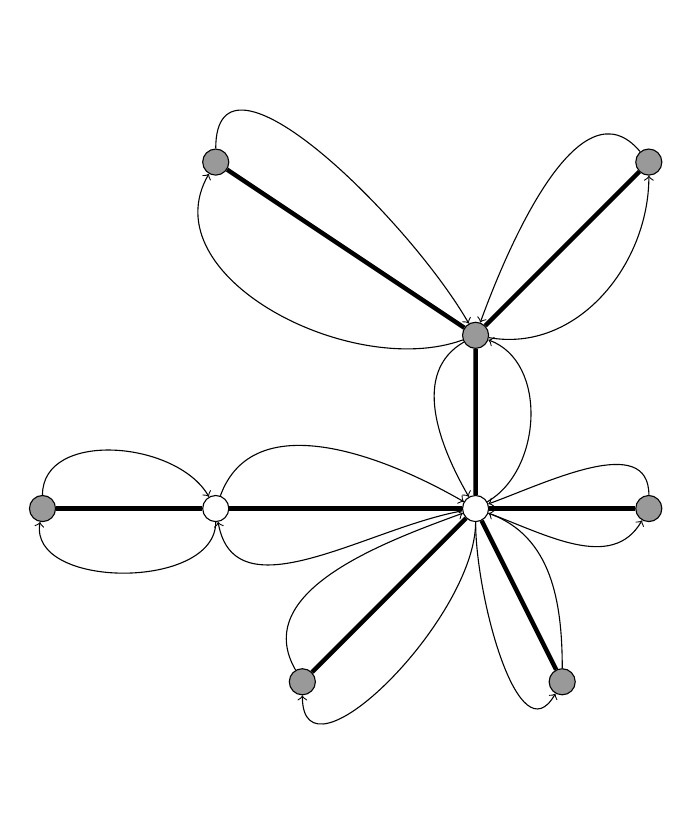
\begin{tikzpicture}[scale=1.1, auto, node distance=2cm,
   node_style/.style={circle,draw=black},
   edge_style/.style={draw=black, ultra thick}]

    \node[node_style, fill=black!40] (v1) at (0,4) {};
    \node[node_style, fill=black!40] (v2) at (-2, 0) {};
    \node[node_style, fill=black!40] (v3) at (1,-2)  {};
    \node[node_style, fill=black!40] (v4) at (4,-2)  {};

    \node[node_style] (v5) at (3,0) {};
    \node[node_style, fill=black!40] (v10) at (5,0) {};
    \node[node_style, fill=black!40] (v11) at (5,4) {};
    \node[node_style] (v6) at (0,0)  {};
    \node[node_style, fill=black!40] (v9) at (3,2)  {};
    \draw[edge_style]  (v2) edge node{} (v6);
    \draw[edge_style]  (v11) edge node{} (v9);
    \draw[edge_style]  (v10) edge node{} (v5);
    \draw[edge_style]  (v1) edge node{} (v9);
    \draw[edge_style]  (v6) edge node{} (v5);
    \draw[edge_style]  (v4) edge node{} (v5);
    \draw[edge_style]  (v3) edge node{} (v5);
    \draw[edge_style]  (v5) edge node{} (v9);
    \draw [black, ->] (v2) to[out=90,in=120] (v6);
    \draw [black, ->] (v6) to[out=-90,in=-100] (v2);
    \draw [black, ->] (v11) to[out=130,in=70] (v9);
    \draw [black, ->] (v9) to[out=-10,in=-90] (v11);
    \draw [black, ->] (v10) to[out=90,in=20] (v5);
    \draw [black, ->] (v5) to[out=-20,in=-120] (v10);
    \draw [black, ->] (v1) to[out=90,in=120] (v9);
    \draw [black, ->] (v9) to[out=200,in=-120] (v1);
    \draw [black, ->] (v6) to[out=70,in=150] (v5);
    \draw [black, ->] (v5) to[out=190,in=-80] (v6);
    \draw [black, ->] (v4) to[out=90,in=-20] (v5);
    \draw [black, ->] (v5) to[out=-90,in=-120] (v4);
    \draw [black, ->] (v3) to[out=120,in=200] (v5);
    \draw [black, ->] (v5) to[out=-90,in=-90] (v3);
    \draw [black, ->] (v9) to[out=210,in=120] (v5);
    \draw [black, ->] (v5) to[out=30,in=-20] (v9);
    \end{tikzpicture}


\end{subfigure}
\end{center}
\caption{Eulerian graph by doubling of edges of Steiner tree.}
% \label{fig:test}
\end{figure}


\begin{figure}
\begin{center}
\begin{subfigure}{.5\textwidth}

  \centering
  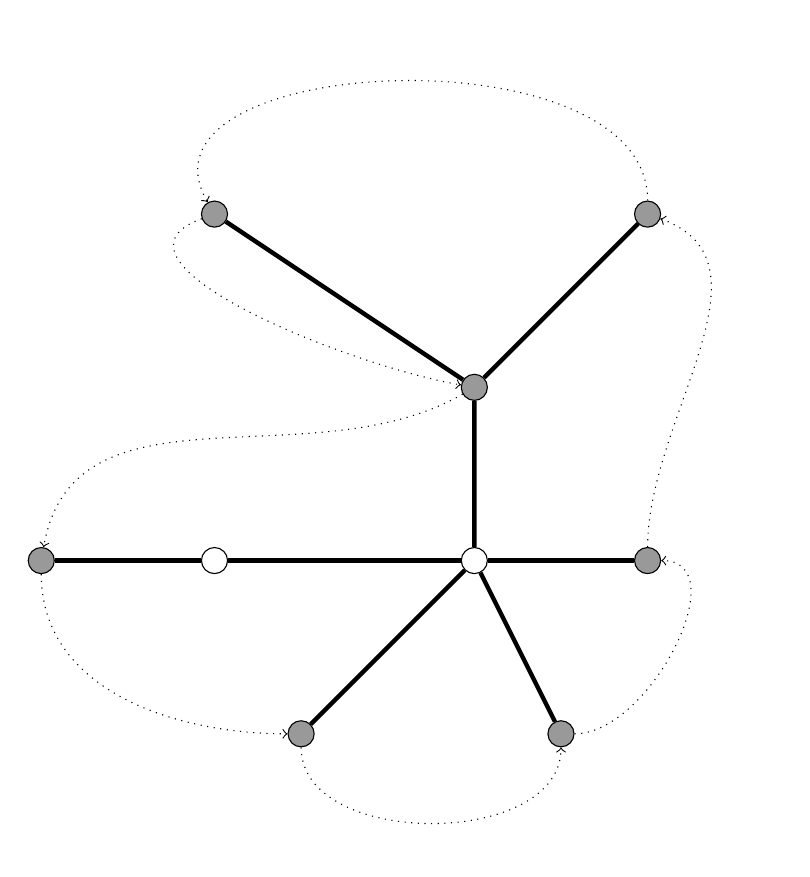
\begin{tikzpicture}[scale=1.1, auto, node distance=2cm,
   node_style/.style={circle,draw=black},
   edge_style/.style={draw=black, ultra thick}]

    \node[node_style, fill=black!40] (v1) at (0,4) {};
    \node[node_style, fill=black!40] (v2) at (-2, 0) {};
    \node[node_style, fill=black!40] (v3) at (1,-2)  {};
    \node[node_style, fill=black!40] (v4) at (4,-2)  {};

    \node[node_style] (v5) at (3,0) {};
    \node[node_style, fill=black!40] (v10) at (5,0) {};
    \node[node_style, fill=black!40] (v11) at (5,4) {};
    \node[node_style] (v6) at (0,0)  {};
    \node[node_style, fill=black!40] (v9) at (3,2)  {};
    \draw[edge_style]  (v2) edge node{} (v6);
    \draw[edge_style]  (v11) edge node{} (v9);
    \draw[edge_style]  (v10) edge node{} (v5);
    \draw[edge_style]  (v1) edge node{} (v9);
    \draw[edge_style]  (v6) edge node{} (v5);
    \draw[edge_style]  (v4) edge node{} (v5);
    \draw[edge_style]  (v3) edge node{} (v5);
    \draw[edge_style]  (v5) edge node{} (v9);
    \draw [black, ->,dotted] (v2) to[out=-90,in=180] (v3);
    % \draw [black, ->,dotted] (v6) to[out=-90,in=-100] (v2);
    % \draw [black, ->,dotted] (v11) to[out=110,in=70] (v9);
    % \draw [black, ->,dotted] (v9) to[out=-10,in=-120] (v11);
    \draw [black, ->,dotted] (v10) to[out=90,in=-20] (v11);
    % \draw [black, ->,dotted] (v5) to[out=-20,in=-120] (v10);
    \draw [black, ->,dotted] (v11) to[out=90,in=120] (v1);
    \draw [black, ->,dotted] (v1) to[out=200,in=170] (v9);
    % \draw [black, ->,dotted] (v6) to[out=70,in=150] (v5);
    % \draw [black, ->,dotted] (v5) to[out=190,in=-80] (v6);
    \draw [black, ->,dotted] (v4) to[out=0,in=0] (v10);
    % \draw [black, ->,dotted] (v5) to[out=-90,in=-120] (v4);
    \draw [black, ->,dotted] (v3) to[out=-90,in=-90] (v4);
    % \draw [black, ->,dotted] (v5) to[out=-90,in=-90] (v3);
    \draw [black, ->,dotted] (v9) to[out=210,in=80] (v2);
    % \draw [black, ->,dotted] (v5) to[out=30,in=-20] (v9);
    \end{tikzpicture}

  
  % \includegraphics[width=.4\linewidth]{image1}
  % \caption{Terminal steiner tree of a Graph G}
  % \label{fig:sub2}
\end{subfigure}
\end{center}
\caption{Hamiltonian Cycle that cover all the Terminals of Steiner tree}
% \label{fig:test}
\end{figure}


\subsection{Tight Analysis of Approximation Ratio}

\begin{lemma} \label{hitsel}
Let $T$ be a tree with $n$ $\geq$ 1 edges. Then, there exists a loop $L$ in $T$, $(v_1,v_2,v_3 \dots, v_{2n})$, where every vertex $v_i$ in tree is in between 1 $\leq$ i $\leq$ 2$n$, such that $(i)$ every edge in $T$ appears exactly twice in the loop, $(ii)$ every leaf vertices in $T$ appears exactly once in the sequence, $(v_1,v_2,v_3 \dots, v_{2n})$ and if $v_i$ and $v_j$ are two leaves in the loop, with no other leaf between them then, $(v_i,v_{i+1},v_{i+2} \dots, v_j)$ is a simple path.
\end{lemma}

\textbf{proof.} Using induction we can proof this lemma, let $n$ = 1, let $\{v_1,v_2 \}$ be the vertices in $T$ that satisfying the above two conditions, if we have a loop $v_1 , v_2, v_1$, let take this as true for $n$= $m$. We have to proof true for $n$ = $m$ + $1$.\\
For $n$ = $m$ + 1, let $v_p$ be the leaf in $T$ and $\{v_p,v_q\}$ be the edge connecting to the $v_p$. Now construct a new tree $T'$, removing the edges $\{v_p,v_q\}$ and the vertex $v_p$ from $T$. $T'$ satisfies the above two condition because $T'$ have n = m edges. Replacing the first appearance of $v_q$ in the loop by $v_q, v_p, v_q$, the lemma then follows.

The Steiner tree produced by above heuristic algorithm is not necessarily minimal. However, it will be shown that the total distance $D_H$(distance of Steiner tree) will not be very far from the $D_{MIN}$, $D_{MIN}$ is the total distance of the minimum Steiner tree.

\begin{lemma} \label{hitsel}
Let $P'$ be the path after removing the longest sub path from the loop $L$, l is the number of leaves in the $OPT$. The total distance of $P'$ is no more than $\big( 1 - \frac{1}{l}\Big)$ times the total distance of $L$.
\end{lemma}

\textbf{Proof.} Let the total distance of the path $P'$ be $D_H$ and $D_{MIN}$ is the total distance of $L$. l leaves appears exactly once in the $L$ that is given by the above lemma, so length of the each subpath will be $\frac{D_{MIN}}{l}$. So length of the longest sub path will be atleast $\frac{D_{MIN}}{l}$.

\begin{center}
 
  $D_H$ $\leq$ $D_{MIN}$ - $\frac{D_{MIN}}{l}$\\
  $D_H$  $\leq$ $D_{MIN}\Big(1- \frac{1}{l} \Big)$ \\

\end{center}
 
 Suppose that every edge in $OPT$ appears at least once in the $P'$. If not, means that edge appears two times in the longest subpath. It follows contradiction because in longest sub path, every edge appears one time only.
 Every edge in $OPT$ appears exactly once in $L$ and every leaf in $OPT$ appears exactly twice in $L$.


 \begin{center}
 $D_H$  $\leq$ $D_{MIN}\Big(1- \frac{1}{l} \Big)$\\
 $D_H$  $\leq$ 2$cost(OPT)\Big(1- \frac{1}{l} \Big)$
 \end{center}

On the other hand, distance of tree  $D_H$ $\geq$ cost of the $G_1$ form in the step 2rd of algorithm because shortest paths are taken in $G_1$, but not in path $P'$. $cost(G_1) \geq$ the cost of the minimum spanning tree of $G_1$, because any spanning tree cost is more than cost of minimum spanning tree. $cost(MST of G_1) \geq cost(T)$ because of removing unnecessary edges from $G_1$. 
 
 \begin{center}
 $cost(T)$  $\leq$ 2$cost(OPT)\Big(1- \frac{1}{l} \Big)$\\
 $D_H$  $\leq$ 2$D_{MIN}\Big(1- \frac{1}{l} \Big)$

 \end{center} 


